\section{Task}
\label{sec:task}

\begin{figure}[h!] 
	\centering
	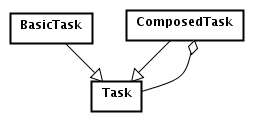
\includegraphics[width=0.4\textwidth]{../Milestone1-DomainModel/TaskDetail.png}
	\caption{task and its relations}
	\label{fig:task} 
\end{figure}

Molto probabilmente il concetto di \emph{Task} esiste gia nell'attuale
versione di \textbf{PMango 2.2.0}. Quello che abbiamo pensato \`e di introdurre
un \emph{glue layer} che ci permette di non apportare modifiche al codice
esistente di mango, ma lavorare con uno strato di intermezzo per essere il meno
intrusivi possibile e poter portare avanti il lavoro dipendendo solo dalle
nostri oggetti, facendo il minor riferimento al codice gia esistente.

Vogliamo rendere trasparente il concetto che un \emph{Task} sia un attivit\`a
singola (non scomponibile in sottoattivit\`a) che una attivit\`a scomposta. 

Costruiamo la relazione $\rightarrow$ che lega questi due concetti:
\begin{itemize}
  \item \emph{BasicTask} $\rightarrow$ attivit\`a di base, non ulteriormente
  scomponibili
  \item \emph{ComposedTask} $\rightarrow$ attivit\`a che sono composte da sotto
  attivit\`a
\end{itemize}
In questo modo possiamo trattare questi due tipi di attivit\`a in modo
interscambiabile e del tutto trasparente. Usando l'astrazione \emph{Task} non
ci importa se abbiamo una attivit\`a base o composta, in quanto cosi le abbiamo
portate ad avere interfaccie compatibili.
